\documentclass{article}
\usepackage{amsmath, amssymb}
\usepackage{tikz}
\begin{document}

\title{Rangkuman Teori Graf}
\author{Teosofi Hidayah Agung}
\date{5002221132}
\maketitle

Dalam teori graf, sebuah graf  terdiri dari himpunan simpul  dan himpunan sisi  yang menghubungkan pasangan simpul. Jika sisi memiliki arah, maka graf disebut sebagai graf berarah, sedangkan jika tidak memiliki arah, disebut sebagai graf tak berarah. Sebuah graf disebut sederhana jika tidak memiliki sisi ganda maupun loop.

$V$ disebut himpunan titik dan $E$ disebut himpunan sisi dari graf $G$. Setiap sisi di $V$ menghubungkan dua titik dari $V$. Istilah lain dari titik adalah \textit{simpul} (\textit{nodes}) dan istilah lain dari sisi adalah \textit{garis} (\textit{lines}).

Gambar di bawah ini menunjukkan sebuah graf $G = (V,E)$ dengan himpunan titik
$
V = \{ v_1, v_2, v_3, v_4 \}
$
dan himpunan sisi
$
E = \{ (v_1, v_2), (v_1, v_3), (v_2, v_4), (v_3, v_4) \}.
$

\begin{center}
    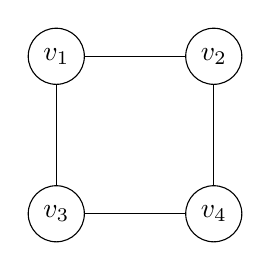
\begin{tikzpicture}
        % Nodes
        \node[draw, circle] (v1) at (0,2) {$v_1$};
        \node[draw, circle] (v2) at (2,2) {$v_2$};
        \node[draw, circle] (v3) at (0,0) {$v_3$};
        \node[draw, circle] (v4) at (2,0) {$v_4$};

        % Edges
        \draw (v1) -- (v2);
        \draw (v1) -- (v3);
        \draw (v2) -- (v4);
        \draw (v3) -- (v4);
    \end{tikzpicture}
\end{center}

Himpunan sisi
$
E = \{ (v_1, v_2), (v_1, v_3), (v_2, v_4), (v_3, v_4) \}
$
dapat ditulis dalam bentuk lain yang lebih singkat, yaitu
$  
E = \{ v_1 v_2, v_1 v_3, v_2 v_4, v_3 v_4 \}
$
atau
$
E = \{ v_2 v_1, v_3 v_1, v_4 v_2, v_4 v_3 \}.
$

Setiap simpul dalam graf memiliki derajat yang menyatakan jumlah sisi yang terhubung dengannya. Pada graf berarah, derajat ini terbagi menjadi derajat masuk dan derajat keluar. Berdasarkan struktur dan hubungan antar simpulnya, graf dapat memiliki berbagai jenis, seperti graf lengkap yang memiliki sisi antara setiap pasangan simpul, graf bipartit yang dapat dipisahkan menjadi dua himpunan tanpa sisi dalam satu himpunan, graf rantai yang berupa jalur linear, serta graf siklus yang memiliki lintasan tertutup.

Jalur dalam graf adalah urutan simpul yang terhubung oleh sisi, dan sebuah jalur disebut sederhana jika tidak ada simpul yang berulang. Beberapa jalur khusus adalah jalur Hamilton yang melewati setiap simpul tepat satu kali dan jalur Euler yang melewati setiap sisi tepat satu kali. Jika jalur tersebut membentuk lintasan tertutup, maka disebut siklus Hamilton atau siklus Euler.

Graf dapat direpresentasikan menggunakan matriks ketetanggaan, di mana elemen-elemen matriks menunjukkan ada atau tidaknya sisi antara dua simpul, atau menggunakan daftar ketetanggaan yang mencatat setiap simpul beserta tetangganya.

Dalam analisis graf, berbagai algoritma digunakan untuk eksplorasi dan optimasi, seperti algoritma pencarian Breadth-First Search (BFS) dan Depth-First Search (DFS). Untuk menemukan jalur terpendek, algoritma Dijkstra digunakan dalam graf berbobot positif, sementara algoritma Bellman-Ford dapat menangani bobot negatif, dan algoritma Floyd-Warshall mencari jalur terpendek antara semua pasangan simpul. Selain itu, dalam menentukan pohon merentang minimum, algoritma Prim dan Kruskal sering digunakan untuk menemukan subgraf pohon dengan total bobot sisi minimum yang mencakup semua simpul tanpa membentuk siklus.

Pohon adalah jenis graf khusus yang bersifat terhubung dan tidak memiliki siklus. Sebuah pohon dengan  simpul selalu memiliki tepat  sisi. Pohon sering digunakan dalam struktur data dan algoritma karena sifat hierarkisnya, serta memiliki berbagai jenis seperti pohon biner, di mana setiap simpul memiliki paling banyak dua anak. Selain itu, pohon juga menjadi dasar dalam konsep pohon merentang minimum yang digunakan dalam jaringan dan optimasi.\\

\noindent\textbf{Referensi}:
\begin{enumerate}
  \item Douglas B. West - Introduction to Graph Theory
  \item Reinhard Diestel - Graph Theory
  \item Gary Chartrand \& Ping Zhang - A First Course in Graph Theory
  \item Jonathan L. Gross \& Jay Yellen - Graph Theory and Its Applications
  \item Bondy \& Murty - Graph Theory with Applications
\end{enumerate}

\end{document}

